\documentclass[1p]{elsarticle_modified}
%\bibliographystyle{elsarticle-num}

%\usepackage[colorlinks]{hyperref}
%\usepackage{abbrmath_seonhwa} %\Abb, \Ascr, \Acal ,\Abf, \Afrak
\usepackage{amsfonts}
\usepackage{amssymb}
\usepackage{amsmath}
\usepackage{amsthm}
\usepackage{scalefnt}
\usepackage{amsbsy}
\usepackage{kotex}
\usepackage{caption}
\usepackage{subfig}
\usepackage{color}
\usepackage{graphicx}
\usepackage{xcolor} %% white, black, red, green, blue, cyan, magenta, yellow
\usepackage{float}
\usepackage{setspace}
\usepackage{hyperref}

\usepackage{tikz}
\usetikzlibrary{arrows}

\usepackage{multirow}
\usepackage{array} % fixed length table
\usepackage{hhline}

%%%%%%%%%%%%%%%%%%%%%
\makeatletter
\renewcommand*\env@matrix[1][\arraystretch]{%
	\edef\arraystretch{#1}%
	\hskip -\arraycolsep
	\let\@ifnextchar\new@ifnextchar
	\array{*\c@MaxMatrixCols c}}
\makeatother %https://tex.stackexchange.com/questions/14071/how-can-i-increase-the-line-spacing-in-a-matrix
%%%%%%%%%%%%%%%

\usepackage[normalem]{ulem}

\newcommand{\msout}[1]{\ifmmode\text{\sout{\ensuremath{#1}}}\else\sout{#1}\fi}
%SOURCE: \msout is \stkout macro in https://tex.stackexchange.com/questions/20609/strikeout-in-math-mode

\newcommand{\cancel}[1]{
	\ifmmode
	{\color{red}\msout{#1}}
	\else
	{\color{red}\sout{#1}}
	\fi
}

\newcommand{\add}[1]{
	{\color{blue}\uwave{#1}}
}

\newcommand{\replace}[2]{
	\ifmmode
	{\color{red}\msout{#1}}{\color{blue}\uwave{#2}}
	\else
	{\color{red}\sout{#1}}{\color{blue}\uwave{#2}}
	\fi
}

\newcommand{\Sol}{\mathcal{S}} %segment
\newcommand{\D}{D} %diagram
\newcommand{\A}{\mathcal{A}} %arc


%%%%%%%%%%%%%%%%%%%%%%%%%%%%%5 test

\def\sl{\operatorname{\textup{SL}}(2,\Cbb)}
\def\psl{\operatorname{\textup{PSL}}(2,\Cbb)}
\def\quan{\mkern 1mu \triangleright \mkern 1mu}

\theoremstyle{definition}
\newtheorem{thm}{Theorem}[section]
\newtheorem{prop}[thm]{Proposition}
\newtheorem{lem}[thm]{Lemma}
\newtheorem{ques}[thm]{Question}
\newtheorem{cor}[thm]{Corollary}
\newtheorem{defn}[thm]{Definition}
\newtheorem{exam}[thm]{Example}
\newtheorem{rmk}[thm]{Remark}
\newtheorem{alg}[thm]{Algorithm}

\newcommand{\I}{\sqrt{-1}}
\begin{document}

%\begin{frontmatter}
%
%\title{Boundary parabolic representations of knots up to 8 crossings}
%
%%% Group authors per affiliation:
%\author{Yunhi Cho} 
%\address{Department of Mathematics, University of Seoul, Seoul, Korea}
%\ead{yhcho@uos.ac.kr}
%
%
%\author{Seonhwa Kim} %\fnref{s_kim}}
%\address{Center for Geometry and Physics, Institute for Basic Science, Pohang, 37673, Korea}
%\ead{ryeona17@ibs.re.kr}
%
%\author{Hyuk Kim}
%\address{Department of Mathematical Sciences, Seoul National University, Seoul 08826, Korea}
%\ead{hyukkim@snu.ac.kr}
%
%\author{Seokbeom Yoon}
%\address{Department of Mathematical Sciences, Seoul National University, Seoul, 08826,  Korea}
%\ead{sbyoon15@snu.ac.kr}
%
%\begin{abstract}
%We find all boundary parabolic representation of knots up to 8 crossings.
%
%\end{abstract}
%\begin{keyword}
%    \MSC[2010] 57M25 
%\end{keyword}
%
%\end{frontmatter}

%\linenumbers
%\tableofcontents
%
\newcommand\colored[1]{\textcolor{white}{\rule[-0.35ex]{0.8em}{1.4ex}}\kern-0.8em\color{red} #1}%
%\newcommand\colored[1]{\textcolor{white}{ #1}\kern-2.17ex	\textcolor{white}{ #1}\kern-1.81ex	\textcolor{white}{ #1}\kern-2.15ex\color{red}#1	}

{\Large $\underline{12n_{0308}~(K12n_{0308})}$}

\setlength{\tabcolsep}{10pt}
\renewcommand{\arraystretch}{1.6}
\vspace{1cm}\begin{tabular}{m{100pt}>{\centering\arraybackslash}m{274pt}}
\multirow{5}{120pt}{
	\centering
	\includegraphics[width=112pt]{../../../GIT/diagram.site/Diagrams/png/2397_12n_0308.png}\\
\ \ \ A knot diagram\footnotemark}&
\allowdisplaybreaks
\textbf{Linearized knot diagam} \\
\cline{2-2}
 &
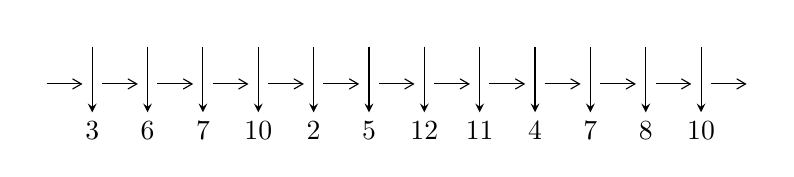
\begin{tikzpicture}[x=20pt, y=17pt]
	% nodes
	\node (C0) at (0, 0) {};
	\node (C1) at (1, 0) {};
	\node (C1U) at (1, +1) {};
	\node (C1D) at (1, -1) {3};

	\node (C2) at (2, 0) {};
	\node (C2U) at (2, +1) {};
	\node (C2D) at (2, -1) {6};

	\node (C3) at (3, 0) {};
	\node (C3U) at (3, +1) {};
	\node (C3D) at (3, -1) {7};

	\node (C4) at (4, 0) {};
	\node (C4U) at (4, +1) {};
	\node (C4D) at (4, -1) {10};

	\node (C5) at (5, 0) {};
	\node (C5U) at (5, +1) {};
	\node (C5D) at (5, -1) {2};

	\node (C6) at (6, 0) {};
	\node (C6U) at (6, +1) {};
	\node (C6D) at (6, -1) {5};

	\node (C7) at (7, 0) {};
	\node (C7U) at (7, +1) {};
	\node (C7D) at (7, -1) {12};

	\node (C8) at (8, 0) {};
	\node (C8U) at (8, +1) {};
	\node (C8D) at (8, -1) {11};

	\node (C9) at (9, 0) {};
	\node (C9U) at (9, +1) {};
	\node (C9D) at (9, -1) {4};

	\node (C10) at (10, 0) {};
	\node (C10U) at (10, +1) {};
	\node (C10D) at (10, -1) {7};

	\node (C11) at (11, 0) {};
	\node (C11U) at (11, +1) {};
	\node (C11D) at (11, -1) {8};

	\node (C12) at (12, 0) {};
	\node (C12U) at (12, +1) {};
	\node (C12D) at (12, -1) {10};
	\node (C13) at (13, 0) {};

	% arrows
	\draw[->,>={angle 60}]
	(C0) edge (C1) (C1) edge (C2) (C2) edge (C3) (C3) edge (C4) (C4) edge (C5) (C5) edge (C6) (C6) edge (C7) (C7) edge (C8) (C8) edge (C9) (C9) edge (C10) (C10) edge (C11) (C11) edge (C12) (C12) edge (C13) ;	\draw[->,>=stealth]
	(C1U) edge (C1D) (C2U) edge (C2D) (C3U) edge (C3D) (C4U) edge (C4D) (C5U) edge (C5D) (C6U) edge (C6D) (C7U) edge (C7D) (C8U) edge (C8D) (C9U) edge (C9D) (C10U) edge (C10D) (C11U) edge (C11D) (C12U) edge (C12D) ;
	\end{tikzpicture} \\
\hhline{~~} \\& 
\textbf{Solving Sequence} \\ \cline{2-2} 
 &
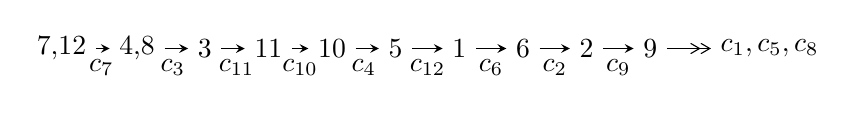
\begin{tikzpicture}[x=23pt, y=7pt]
	% node
	\node (A0) at (-1/8, 0) {7,12};
	\node (A1) at (17/16, 0) {4,8};
	\node (A2) at (17/8, 0) {3};
	\node (A3) at (25/8, 0) {11};
	\node (A4) at (33/8, 0) {10};
	\node (A5) at (41/8, 0) {5};
	\node (A6) at (49/8, 0) {1};
	\node (A7) at (57/8, 0) {6};
	\node (A8) at (65/8, 0) {2};
	\node (A9) at (73/8, 0) {9};
	\node (C1) at (1/2, -1) {$c_{7}$};
	\node (C2) at (13/8, -1) {$c_{3}$};
	\node (C3) at (21/8, -1) {$c_{11}$};
	\node (C4) at (29/8, -1) {$c_{10}$};
	\node (C5) at (37/8, -1) {$c_{4}$};
	\node (C6) at (45/8, -1) {$c_{12}$};
	\node (C7) at (53/8, -1) {$c_{6}$};
	\node (C8) at (61/8, -1) {$c_{2}$};
	\node (C9) at (69/8, -1) {$c_{9}$};
	\node (A10) at (11, 0) {$c_{1},c_{5},c_{8}$};

	% edge
	\draw[->,>=stealth]	
	(A0) edge (A1) (A1) edge (A2) (A2) edge (A3) (A3) edge (A4) (A4) edge (A5) (A5) edge (A6) (A6) edge (A7) (A7) edge (A8) (A8) edge (A9) ;
	\draw[->>,>={angle 60}]	
	(A9) edge (A10);
\end{tikzpicture} \\ 

\end{tabular} \\

\footnotetext{
The image of knot diagram is generated by the software ``\textbf{Draw programme}" developed by Andrew Bartholomew(\url{http://www.layer8.co.uk/maths/draw/index.htm\#Running-draw}), where we modified some parts for our purpose(\url{https://github.com/CATsTAILs/LinksPainter}).
}\phantom \\ \newline 
\centering \textbf{Ideals for irreducible components\footnotemark of $X_{\text{par}}$} 
 
\begin{align*}
I^u_{1}&=\langle 
6 u^{39}+24 u^{38}+\cdots+4 b-9,\;9 u^{39}+30 u^{38}+\cdots+4 a-24,\;u^{40}+4 u^{39}+\cdots-2 u-1\rangle \\
I^u_{2}&=\langle 
b+u,\;a+1,\;u^3- u^2+2 u-1\rangle \\
I^u_{3}&=\langle 
- a u+b,\;u^2 a+a^2- a u+3 u^2+a- u+5,\;u^3- u^2+2 u-1\rangle \\
\\
\end{align*}
\raggedright * 3 irreducible components of $\dim_{\mathbb{C}}=0$, with total 49 representations.\\
\footnotetext{All coefficients of polynomials are rational numbers. But the coefficients are sometimes approximated in decimal forms when there is not enough margin.}
\newpage
\renewcommand{\arraystretch}{1}
\centering \section*{I. $I^u_{1}= \langle 6 u^{39}+24 u^{38}+\cdots+4 b-9,\;9 u^{39}+30 u^{38}+\cdots+4 a-24,\;u^{40}+4 u^{39}+\cdots-2 u-1 \rangle$}
\flushleft \textbf{(i) Arc colorings}\\
\begin{tabular}{m{7pt} m{180pt} m{7pt} m{180pt} }
\flushright $a_{7}=$&$\begin{pmatrix}1\\0\end{pmatrix}$ \\
\flushright $a_{12}=$&$\begin{pmatrix}0\\u\end{pmatrix}$ \\
\flushright $a_{4}=$&$\begin{pmatrix}-\frac{9}{4} u^{39}-\frac{15}{2} u^{38}+\cdots-\frac{37}{4} u+6\\-\frac{3}{2} u^{39}-6 u^{38}+\cdots-\frac{3}{2} u+\frac{9}{4}\end{pmatrix}$ \\
\flushright $a_{8}=$&$\begin{pmatrix}1\\u^2\end{pmatrix}$ \\
\flushright $a_{3}=$&$\begin{pmatrix}-3.75000 u^{39}-13.5000 u^{38}+\cdots-10.7500 u+8.25000\\-\frac{3}{2} u^{39}-6 u^{38}+\cdots-\frac{3}{2} u+\frac{9}{4}\end{pmatrix}$ \\
\flushright $a_{11}=$&$\begin{pmatrix}u\\u^3+u\end{pmatrix}$ \\
\flushright $a_{10}=$&$\begin{pmatrix}u^3+2 u\\u^3+u\end{pmatrix}$ \\
\flushright $a_{5}=$&$\begin{pmatrix}-\frac{11}{4} u^{39}-\frac{17}{2} u^{38}+\cdots-\frac{43}{4} u+7\\-\frac{3}{2} u^{39}-5 u^{38}+\cdots-\frac{5}{2} u+\frac{11}{4}\end{pmatrix}$ \\
\flushright $a_{1}=$&$\begin{pmatrix}- u^7-4 u^5-4 u^3\\- u^7-3 u^5-2 u^3+u\end{pmatrix}$ \\
\flushright $a_{6}=$&$\begin{pmatrix}\frac{1}{2} u^{39}+\frac{7}{4} u^{38}+\cdots-\frac{21}{4} u+\frac{5}{4}\\\frac{1}{4} u^{39}+u^{38}+\cdots-\frac{5}{4} u-\frac{1}{2}\end{pmatrix}$ \\
\flushright $a_{2}=$&$\begin{pmatrix}-\frac{3}{4} u^{39}-\frac{11}{4} u^{38}+\cdots+\frac{13}{2} u+\frac{1}{4}\\-\frac{1}{4} u^{39}- u^{38}+\cdots+\frac{9}{4} u+\frac{1}{2}\end{pmatrix}$ \\
\flushright $a_{9}=$&$\begin{pmatrix}u^2+1\\u^4+2 u^2\end{pmatrix}$\\&\end{tabular}
\flushleft \textbf{(ii) Obstruction class $= -1$}\\~\\
\flushleft \textbf{(iii) Cusp Shapes $= -\frac{9}{2} u^{39}-\frac{37}{2} u^{38}+\cdots-\frac{39}{2} u-\frac{7}{4}$}\\~\\
\newpage\renewcommand{\arraystretch}{1}
\flushleft \textbf{(iv) u-Polynomials at the component}\newline \\
\begin{tabular}{m{50pt}|m{274pt}}
Crossings & \hspace{64pt}u-Polynomials at each crossing \\
\hline $$\begin{aligned}c_{1},c_{6}\end{aligned}$$&$\begin{aligned}
&u^{40}+16 u^{39}+\cdots+14 u+1
\end{aligned}$\\
\hline $$\begin{aligned}c_{2},c_{5}\end{aligned}$$&$\begin{aligned}
&u^{40}+4 u^{39}+\cdots-6 u-1
\end{aligned}$\\
\hline $$\begin{aligned}c_{3}\end{aligned}$$&$\begin{aligned}
&u^{40}-4 u^{39}+\cdots+7 u^2-1
\end{aligned}$\\
\hline $$\begin{aligned}c_{4},c_{9}\end{aligned}$$&$\begin{aligned}
&u^{40}- u^{39}+\cdots+1536 u+512
\end{aligned}$\\
\hline $$\begin{aligned}c_{7},c_{8},c_{11}\end{aligned}$$&$\begin{aligned}
&u^{40}-4 u^{39}+\cdots+2 u-1
\end{aligned}$\\
\hline $$\begin{aligned}c_{10}\end{aligned}$$&$\begin{aligned}
&u^{40}+4 u^{39}+\cdots+7 u-2
\end{aligned}$\\
\hline $$\begin{aligned}c_{12}\end{aligned}$$&$\begin{aligned}
&u^{40}-20 u^{39}+\cdots-2480 u+20513
\end{aligned}$\\
\hline
\end{tabular}\\~\\
\newpage\renewcommand{\arraystretch}{1}
\flushleft \textbf{(v) Riley Polynomials at the component}\newline \\
\begin{tabular}{m{50pt}|m{274pt}}
Crossings & \hspace{64pt}Riley Polynomials at each crossing \\
\hline $$\begin{aligned}c_{1},c_{6}\end{aligned}$$&$\begin{aligned}
&y^{40}+20 y^{39}+\cdots-142 y+1
\end{aligned}$\\
\hline $$\begin{aligned}c_{2},c_{5}\end{aligned}$$&$\begin{aligned}
&y^{40}-16 y^{39}+\cdots-14 y+1
\end{aligned}$\\
\hline $$\begin{aligned}c_{3}\end{aligned}$$&$\begin{aligned}
&y^{40}-64 y^{39}+\cdots-14 y+1
\end{aligned}$\\
\hline $$\begin{aligned}c_{4},c_{9}\end{aligned}$$&$\begin{aligned}
&y^{40}-49 y^{39}+\cdots-655360 y+262144
\end{aligned}$\\
\hline $$\begin{aligned}c_{7},c_{8},c_{11}\end{aligned}$$&$\begin{aligned}
&y^{40}+32 y^{39}+\cdots-22 y+1
\end{aligned}$\\
\hline $$\begin{aligned}c_{10}\end{aligned}$$&$\begin{aligned}
&y^{40}-48 y^{39}+\cdots-109 y+4
\end{aligned}$\\
\hline $$\begin{aligned}c_{12}\end{aligned}$$&$\begin{aligned}
&y^{40}-76 y^{39}+\cdots-22287329974 y+420783169
\end{aligned}$\\
\hline
\end{tabular}\\~\\
\newpage\flushleft \textbf{(vi) Complex Volumes and Cusp Shapes}
$$\begin{array}{c|c|c}  
\text{Solutions to }I^u_{1}& \I (\text{vol} + \sqrt{-1}CS) & \text{Cusp shape}\\
 \hline 
\begin{aligned}
u &= -0.965795\phantom{ +0.000000I} \\
a &= -2.34182\phantom{ +0.000000I} \\
b &= -2.26172\phantom{ +0.000000I}\end{aligned}
 & -14.3054\phantom{ +0.000000I} & -18.4760\phantom{ +0.000000I} \\ \hline\begin{aligned}
u &= \phantom{-}0.139471 + 0.935681 I \\
a &= \phantom{-}0.435322 + 0.697825 I \\
b &= \phantom{-}0.592227 - 0.504649 I\end{aligned}
 & -0.336971 + 0.164971 I & -14.2424 - 0.6515 I \\ \hline\begin{aligned}
u &= \phantom{-}0.139471 - 0.935681 I \\
a &= \phantom{-}0.435322 - 0.697825 I \\
b &= \phantom{-}0.592227 + 0.504649 I\end{aligned}
 & -0.336971 - 0.164971 I & -14.2424 + 0.6515 I \\ \hline\begin{aligned}
u &= -0.938638 + 0.087954 I \\
a &= -2.38096 - 0.31083 I \\
b &= -2.26220 - 0.08234 I\end{aligned}
 & -9.79280 + 8.10641 I & -15.5163 - 4.8945 I \\ \hline\begin{aligned}
u &= -0.938638 - 0.087954 I \\
a &= -2.38096 + 0.31083 I \\
b &= -2.26220 + 0.08234 I\end{aligned}
 & -9.79280 - 8.10641 I & -15.5163 + 4.8945 I \\ \hline\begin{aligned}
u &= -0.916347 + 0.055169 I \\
a &= \phantom{-}2.49555 + 0.21808 I \\
b &= \phantom{-}2.29882 + 0.06216 I\end{aligned}
 & -7.85713 + 2.28541 I & -13.64199 - 0.57988 I \\ \hline\begin{aligned}
u &= -0.916347 - 0.055169 I \\
a &= \phantom{-}2.49555 - 0.21808 I \\
b &= \phantom{-}2.29882 - 0.06216 I\end{aligned}
 & -7.85713 - 2.28541 I & -13.64199 + 0.57988 I \\ \hline\begin{aligned}
u &= -0.119891 + 1.171300 I \\
a &= \phantom{-}1.32469 + 0.51665 I \\
b &= \phantom{-}0.76397 - 1.48966 I\end{aligned}
 & \phantom{-}5.65080 + 4.37709 I & -8.98534 - 1.57605 I \\ \hline\begin{aligned}
u &= -0.119891 - 1.171300 I \\
a &= \phantom{-}1.32469 - 0.51665 I \\
b &= \phantom{-}0.76397 + 1.48966 I\end{aligned}
 & \phantom{-}5.65080 - 4.37709 I & -8.98534 + 1.57605 I \\ \hline\begin{aligned}
u &= -0.075508 + 1.198880 I \\
a &= -1.212150 - 0.270191 I \\
b &= -0.41545 + 1.43282 I\end{aligned}
 & \phantom{-}6.05510 - 1.44432 I & -7.22921 + 3.78916 I\\
 \hline 
 \end{array}$$\newpage$$\begin{array}{c|c|c}  
\text{Solutions to }I^u_{1}& \I (\text{vol} + \sqrt{-1}CS) & \text{Cusp shape}\\
 \hline 
\begin{aligned}
u &= -0.075508 - 1.198880 I \\
a &= -1.212150 + 0.270191 I \\
b &= -0.41545 - 1.43282 I\end{aligned}
 & \phantom{-}6.05510 + 1.44432 I & -7.22921 - 3.78916 I \\ \hline\begin{aligned}
u &= \phantom{-}0.182743 + 1.209970 I \\
a &= -0.361246 - 0.222448 I \\
b &= -0.203140 + 0.477747 I\end{aligned}
 & \phantom{-}2.74721 - 2.07700 I & -5.89369 + 3.03885 I \\ \hline\begin{aligned}
u &= \phantom{-}0.182743 - 1.209970 I \\
a &= -0.361246 + 0.222448 I \\
b &= -0.203140 - 0.477747 I\end{aligned}
 & \phantom{-}2.74721 + 2.07700 I & -5.89369 - 3.03885 I \\ \hline\begin{aligned}
u &= \phantom{-}0.359488 + 1.180450 I \\
a &= \phantom{-}0.169664 + 0.421096 I \\
b &= \phantom{-}0.436088 - 0.351658 I\end{aligned}
 & \phantom{-}1.06997 - 5.73235 I & -12.00000 + 6.50930 I \\ \hline\begin{aligned}
u &= \phantom{-}0.359488 - 1.180450 I \\
a &= \phantom{-}0.169664 - 0.421096 I \\
b &= \phantom{-}0.436088 + 0.351658 I\end{aligned}
 & \phantom{-}1.06997 + 5.73235 I & -12.00000 - 6.50930 I \\ \hline\begin{aligned}
u &= \phantom{-}0.758575 + 0.094110 I \\
a &= \phantom{-}0.049336 - 0.391801 I \\
b &= -0.074297 + 0.292567 I\end{aligned}
 & -2.22421 + 1.66592 I & -15.6530 - 3.4641 I \\ \hline\begin{aligned}
u &= \phantom{-}0.758575 - 0.094110 I \\
a &= \phantom{-}0.049336 + 0.391801 I \\
b &= -0.074297 - 0.292567 I\end{aligned}
 & -2.22421 - 1.66592 I & -15.6530 + 3.4641 I \\ \hline\begin{aligned}
u &= \phantom{-}0.633093 + 0.358144 I \\
a &= \phantom{-}0.135758 - 0.528918 I \\
b &= -0.275376 + 0.286233 I\end{aligned}
 & -1.63533 - 3.53225 I & -15.3501 + 6.0239 I \\ \hline\begin{aligned}
u &= \phantom{-}0.633093 - 0.358144 I \\
a &= \phantom{-}0.135758 + 0.528918 I \\
b &= -0.275376 - 0.286233 I\end{aligned}
 & -1.63533 + 3.53225 I & -15.3501 - 6.0239 I \\ \hline\begin{aligned}
u &= -0.494907 + 1.218760 I \\
a &= -0.89625 - 1.31642 I \\
b &= -2.04796 + 0.44080 I\end{aligned}
 & -6.31623 - 3.01599 I & \phantom{-0.000000 } 0\\
 \hline 
 \end{array}$$\newpage$$\begin{array}{c|c|c}  
\text{Solutions to }I^u_{1}& \I (\text{vol} + \sqrt{-1}CS) & \text{Cusp shape}\\
 \hline 
\begin{aligned}
u &= -0.494907 - 1.218760 I \\
a &= -0.89625 + 1.31642 I \\
b &= -2.04796 - 0.44080 I\end{aligned}
 & -6.31623 + 3.01599 I & \phantom{-0.000000 } 0 \\ \hline\begin{aligned}
u &= -0.457832 + 1.243030 I \\
a &= \phantom{-}0.88954 + 1.38304 I \\
b &= \phantom{-}2.12642 - 0.47253 I\end{aligned}
 & -4.18941 + 2.61474 I & \phantom{-0.000000 } 0 \\ \hline\begin{aligned}
u &= -0.457832 - 1.243030 I \\
a &= \phantom{-}0.88954 - 1.38304 I \\
b &= \phantom{-}2.12642 + 0.47253 I\end{aligned}
 & -4.18941 - 2.61474 I & \phantom{-0.000000 } 0 \\ \hline\begin{aligned}
u &= \phantom{-}0.285992 + 1.310300 I \\
a &= -0.053918 - 0.293250 I \\
b &= -0.368826 + 0.154516 I\end{aligned}
 & \phantom{-}2.18000 - 2.07454 I & \phantom{-0.000000 } 0 \\ \hline\begin{aligned}
u &= \phantom{-}0.285992 - 1.310300 I \\
a &= -0.053918 + 0.293250 I \\
b &= -0.368826 - 0.154516 I\end{aligned}
 & \phantom{-}2.18000 + 2.07454 I & \phantom{-0.000000 } 0 \\ \hline\begin{aligned}
u &= -0.480023 + 1.304310 I \\
a &= -0.77326 - 1.37509 I \\
b &= -2.16472 + 0.34850 I\end{aligned}
 & -10.25510 + 5.14488 I & \phantom{-0.000000 } 0 \\ \hline\begin{aligned}
u &= -0.480023 - 1.304310 I \\
a &= -0.77326 + 1.37509 I \\
b &= -2.16472 - 0.34850 I\end{aligned}
 & -10.25510 - 5.14488 I & \phantom{-0.000000 } 0 \\ \hline\begin{aligned}
u &= \phantom{-}0.146448 + 1.384710 I \\
a &= -0.301378 + 0.307270 I \\
b &= \phantom{-}0.469617 + 0.372324 I\end{aligned}
 & \phantom{-}4.81791 - 1.66817 I & \phantom{-0.000000 } 0 \\ \hline\begin{aligned}
u &= \phantom{-}0.146448 - 1.384710 I \\
a &= -0.301378 - 0.307270 I \\
b &= \phantom{-}0.469617 - 0.372324 I\end{aligned}
 & \phantom{-}4.81791 + 1.66817 I & \phantom{-0.000000 } 0 \\ \hline\begin{aligned}
u &= -0.427217 + 1.328920 I \\
a &= \phantom{-}0.72481 + 1.49260 I \\
b &= \phantom{-}2.29320 - 0.32556 I\end{aligned}
 & -3.52880 + 7.09218 I & \phantom{-0.000000 } 0\\
 \hline 
 \end{array}$$\newpage$$\begin{array}{c|c|c}  
\text{Solutions to }I^u_{1}& \I (\text{vol} + \sqrt{-1}CS) & \text{Cusp shape}\\
 \hline 
\begin{aligned}
u &= -0.427217 - 1.328920 I \\
a &= \phantom{-}0.72481 - 1.49260 I \\
b &= \phantom{-}2.29320 + 0.32556 I\end{aligned}
 & -3.52880 - 7.09218 I & \phantom{-0.000000 } 0 \\ \hline\begin{aligned}
u &= -0.43256 + 1.35367 I \\
a &= -0.66257 - 1.47304 I \\
b &= -2.28062 + 0.25972 I\end{aligned}
 & -5.27211 + 13.00920 I & \phantom{-0.000000 } 0 \\ \hline\begin{aligned}
u &= -0.43256 - 1.35367 I \\
a &= -0.66257 + 1.47304 I \\
b &= -2.28062 - 0.25972 I\end{aligned}
 & -5.27211 - 13.00920 I & \phantom{-0.000000 } 0 \\ \hline\begin{aligned}
u &= \phantom{-}0.19436 + 1.41468 I \\
a &= \phantom{-}0.190363 - 0.356157 I \\
b &= -0.540845 - 0.200080 I\end{aligned}
 & \phantom{-}4.09613 - 6.42410 I & \phantom{-0.000000 } 0 \\ \hline\begin{aligned}
u &= \phantom{-}0.19436 - 1.41468 I \\
a &= \phantom{-}0.190363 + 0.356157 I \\
b &= -0.540845 + 0.200080 I\end{aligned}
 & \phantom{-}4.09613 + 6.42410 I & \phantom{-0.000000 } 0 \\ \hline\begin{aligned}
u &= \phantom{-}0.269571 + 0.358650 I \\
a &= -0.373006 + 0.916266 I \\
b &= \phantom{-}0.429170 - 0.113220 I\end{aligned}
 & -0.650305 + 0.185166 I & -12.44941 + 0.70433 I \\ \hline\begin{aligned}
u &= \phantom{-}0.269571 - 0.358650 I \\
a &= -0.373006 - 0.916266 I \\
b &= \phantom{-}0.429170 + 0.113220 I\end{aligned}
 & -0.650305 - 0.185166 I & -12.44941 - 0.70433 I \\ \hline\begin{aligned}
u &= \phantom{-}0.334754\phantom{ +0.000000I} \\
a &= -0.815567\phantom{ +0.000000I} \\
b &= \phantom{-}0.273014\phantom{ +0.000000I}\end{aligned}
 & -0.669605\phantom{ +0.000000I} & -14.6520\phantom{ +0.000000I} \\ \hline\begin{aligned}
u &= -0.311291 + 0.046384 I \\
a &= \phantom{-}0.17839 + 3.50865 I \\
b &= \phantom{-}0.218277 + 1.083940 I\end{aligned}
 & \phantom{-}2.49750 - 2.73965 I & -2.44237 + 2.28441 I \\ \hline\begin{aligned}
u &= -0.311291 - 0.046384 I \\
a &= \phantom{-}0.17839 - 3.50865 I \\
b &= \phantom{-}0.218277 - 1.083940 I\end{aligned}
 & \phantom{-}2.49750 + 2.73965 I & -2.44237 - 2.28441 I\\
 \hline 
 \end{array}$$\newpage\newpage\renewcommand{\arraystretch}{1}
\centering \section*{II. $I^u_{2}= \langle b+u,\;a+1,\;u^3- u^2+2 u-1 \rangle$}
\flushleft \textbf{(i) Arc colorings}\\
\begin{tabular}{m{7pt} m{180pt} m{7pt} m{180pt} }
\flushright $a_{7}=$&$\begin{pmatrix}1\\0\end{pmatrix}$ \\
\flushright $a_{12}=$&$\begin{pmatrix}0\\u\end{pmatrix}$ \\
\flushright $a_{4}=$&$\begin{pmatrix}-1\\- u\end{pmatrix}$ \\
\flushright $a_{8}=$&$\begin{pmatrix}1\\u^2\end{pmatrix}$ \\
\flushright $a_{3}=$&$\begin{pmatrix}- u-1\\- u\end{pmatrix}$ \\
\flushright $a_{11}=$&$\begin{pmatrix}u\\u^2- u+1\end{pmatrix}$ \\
\flushright $a_{10}=$&$\begin{pmatrix}u^2+1\\u^2- u+1\end{pmatrix}$ \\
\flushright $a_{5}=$&$\begin{pmatrix}-1\\- u\end{pmatrix}$ \\
\flushright $a_{1}=$&$\begin{pmatrix}-1\\0\end{pmatrix}$ \\
\flushright $a_{6}=$&$\begin{pmatrix}- u+1\\- u^2\end{pmatrix}$ \\
\flushright $a_{2}=$&$\begin{pmatrix}- u^2- u-1\\- u^2\end{pmatrix}$ \\
\flushright $a_{9}=$&$\begin{pmatrix}u^2+1\\u^2- u+1\end{pmatrix}$\\&\end{tabular}
\flushleft \textbf{(ii) Obstruction class $= 1$}\\~\\
\flushleft \textbf{(iii) Cusp Shapes $= -7 u^2+8 u-20$}\\~\\
\newpage\renewcommand{\arraystretch}{1}
\flushleft \textbf{(iv) u-Polynomials at the component}\newline \\
\begin{tabular}{m{50pt}|m{274pt}}
Crossings & \hspace{64pt}u-Polynomials at each crossing \\
\hline $$\begin{aligned}c_{1},c_{3},c_{7}\\c_{8}\end{aligned}$$&$\begin{aligned}
&u^3- u^2+2 u-1
\end{aligned}$\\
\hline $$\begin{aligned}c_{2}\end{aligned}$$&$\begin{aligned}
&u^3+u^2-1
\end{aligned}$\\
\hline $$\begin{aligned}c_{4},c_{9}\end{aligned}$$&$\begin{aligned}
&u^3
\end{aligned}$\\
\hline $$\begin{aligned}c_{5},c_{10},c_{12}\end{aligned}$$&$\begin{aligned}
&u^3- u^2+1
\end{aligned}$\\
\hline $$\begin{aligned}c_{6},c_{11}\end{aligned}$$&$\begin{aligned}
&u^3+u^2+2 u+1
\end{aligned}$\\
\hline
\end{tabular}\\~\\
\newpage\renewcommand{\arraystretch}{1}
\flushleft \textbf{(v) Riley Polynomials at the component}\newline \\
\begin{tabular}{m{50pt}|m{274pt}}
Crossings & \hspace{64pt}Riley Polynomials at each crossing \\
\hline $$\begin{aligned}c_{1},c_{3},c_{6}\\c_{7},c_{8},c_{11}\end{aligned}$$&$\begin{aligned}
&y^3+3 y^2+2 y-1
\end{aligned}$\\
\hline $$\begin{aligned}c_{2},c_{5},c_{10}\\c_{12}\end{aligned}$$&$\begin{aligned}
&y^3- y^2+2 y-1
\end{aligned}$\\
\hline $$\begin{aligned}c_{4},c_{9}\end{aligned}$$&$\begin{aligned}
&y^3
\end{aligned}$\\
\hline
\end{tabular}\\~\\
\newpage\flushleft \textbf{(vi) Complex Volumes and Cusp Shapes}
$$\begin{array}{c|c|c}  
\text{Solutions to }I^u_{2}& \I (\text{vol} + \sqrt{-1}CS) & \text{Cusp shape}\\
 \hline 
\begin{aligned}
u &= \phantom{-}0.215080 + 1.307140 I \\
a &= -1.00000\phantom{ +0.000000I} \\
b &= -0.215080 - 1.307140 I\end{aligned}
 & \phantom{-}6.04826 - 5.65624 I & -6.64285 + 6.52117 I \\ \hline\begin{aligned}
u &= \phantom{-}0.215080 - 1.307140 I \\
a &= -1.00000\phantom{ +0.000000I} \\
b &= -0.215080 + 1.307140 I\end{aligned}
 & \phantom{-}6.04826 + 5.65624 I & -6.64285 - 6.52117 I \\ \hline\begin{aligned}
u &= \phantom{-}0.569840\phantom{ +0.000000I} \\
a &= -1.00000\phantom{ +0.000000I} \\
b &= -0.569840\phantom{ +0.000000I}\end{aligned}
 & -2.22691\phantom{ +0.000000I} & -17.7140\phantom{ +0.000000I}\\
 \hline 
 \end{array}$$\newpage\newpage\renewcommand{\arraystretch}{1}
\centering \section*{III. $I^u_{3}= \langle - a u+b,\;u^2 a+a^2- a u+3 u^2+a- u+5,\;u^3- u^2+2 u-1 \rangle$}
\flushleft \textbf{(i) Arc colorings}\\
\begin{tabular}{m{7pt} m{180pt} m{7pt} m{180pt} }
\flushright $a_{7}=$&$\begin{pmatrix}1\\0\end{pmatrix}$ \\
\flushright $a_{12}=$&$\begin{pmatrix}0\\u\end{pmatrix}$ \\
\flushright $a_{4}=$&$\begin{pmatrix}a\\a u\end{pmatrix}$ \\
\flushright $a_{8}=$&$\begin{pmatrix}1\\u^2\end{pmatrix}$ \\
\flushright $a_{3}=$&$\begin{pmatrix}a u+a\\a u\end{pmatrix}$ \\
\flushright $a_{11}=$&$\begin{pmatrix}u\\u^2- u+1\end{pmatrix}$ \\
\flushright $a_{10}=$&$\begin{pmatrix}u^2+1\\u^2- u+1\end{pmatrix}$ \\
\flushright $a_{5}=$&$\begin{pmatrix}a\\a u\end{pmatrix}$ \\
\flushright $a_{1}=$&$\begin{pmatrix}-1\\0\end{pmatrix}$ \\
\flushright $a_{6}=$&$\begin{pmatrix}- a u+2 u^2+a- u+4\\- u^2 a+a u+u^2- u+2\end{pmatrix}$ \\
\flushright $a_{2}=$&$\begin{pmatrix}- u^2 a+3 u^2+a-2 u+4\\- u^2 a+a u+u^2- u+2\end{pmatrix}$ \\
\flushright $a_{9}=$&$\begin{pmatrix}u^2+1\\u^2- u+1\end{pmatrix}$\\&\end{tabular}
\flushleft \textbf{(ii) Obstruction class $= 1$}\\~\\
\flushleft \textbf{(iii) Cusp Shapes $= -3 u^2 a-3 a u-2 u^2+a+4 u-19$}\\~\\
\newpage\renewcommand{\arraystretch}{1}
\flushleft \textbf{(iv) u-Polynomials at the component}\newline \\
\begin{tabular}{m{50pt}|m{274pt}}
Crossings & \hspace{64pt}u-Polynomials at each crossing \\
\hline $$\begin{aligned}c_{1},c_{3},c_{7}\\c_{8}\end{aligned}$$&$\begin{aligned}
&(u^3- u^2+2 u-1)^2
\end{aligned}$\\
\hline $$\begin{aligned}c_{2}\end{aligned}$$&$\begin{aligned}
&(u^3+u^2-1)^2
\end{aligned}$\\
\hline $$\begin{aligned}c_{4},c_{9}\end{aligned}$$&$\begin{aligned}
&u^6
\end{aligned}$\\
\hline $$\begin{aligned}c_{5},c_{10},c_{12}\end{aligned}$$&$\begin{aligned}
&(u^3- u^2+1)^2
\end{aligned}$\\
\hline $$\begin{aligned}c_{6},c_{11}\end{aligned}$$&$\begin{aligned}
&(u^3+u^2+2 u+1)^2
\end{aligned}$\\
\hline
\end{tabular}\\~\\
\newpage\renewcommand{\arraystretch}{1}
\flushleft \textbf{(v) Riley Polynomials at the component}\newline \\
\begin{tabular}{m{50pt}|m{274pt}}
Crossings & \hspace{64pt}Riley Polynomials at each crossing \\
\hline $$\begin{aligned}c_{1},c_{3},c_{6}\\c_{7},c_{8},c_{11}\end{aligned}$$&$\begin{aligned}
&(y^3+3 y^2+2 y-1)^2
\end{aligned}$\\
\hline $$\begin{aligned}c_{2},c_{5},c_{10}\\c_{12}\end{aligned}$$&$\begin{aligned}
&(y^3- y^2+2 y-1)^2
\end{aligned}$\\
\hline $$\begin{aligned}c_{4},c_{9}\end{aligned}$$&$\begin{aligned}
&y^6
\end{aligned}$\\
\hline
\end{tabular}\\~\\
\newpage\flushleft \textbf{(vi) Complex Volumes and Cusp Shapes}
$$\begin{array}{c|c|c}  
\text{Solutions to }I^u_{3}& \I (\text{vol} + \sqrt{-1}CS) & \text{Cusp shape}\\
 \hline 
\begin{aligned}
u &= \phantom{-}0.215080 + 1.307140 I \\
a &= \phantom{-}0.947279 + 0.320410 I \\
b &= -0.215080 + 1.307140 I\end{aligned}
 & \phantom{-}6.04826\phantom{ +0.000000I} & -7.95781 + 0.50299 I \\ \hline\begin{aligned}
u &= \phantom{-}0.215080 + 1.307140 I \\
a &= -0.069840 + 0.424452 I \\
b &= -0.569840\phantom{ +0.000000I}\end{aligned}
 & \phantom{-}1.91067 - 2.82812 I & -12.8076 + 6.7630 I \\ \hline\begin{aligned}
u &= \phantom{-}0.215080 - 1.307140 I \\
a &= \phantom{-}0.947279 - 0.320410 I \\
b &= -0.215080 - 1.307140 I\end{aligned}
 & \phantom{-}6.04826\phantom{ +0.000000I} & -7.95781 - 0.50299 I \\ \hline\begin{aligned}
u &= \phantom{-}0.215080 - 1.307140 I \\
a &= -0.069840 - 0.424452 I \\
b &= -0.569840\phantom{ +0.000000I}\end{aligned}
 & \phantom{-}1.91067 + 2.82812 I & -12.8076 - 6.7630 I \\ \hline\begin{aligned}
u &= \phantom{-}0.569840\phantom{ +0.000000I} \\
a &= -0.37744 + 2.29387 I \\
b &= -0.215080 + 1.307140 I\end{aligned}
 & \phantom{-}1.91067 + 2.82812 I & -16.7346 - 3.8621 I \\ \hline\begin{aligned}
u &= \phantom{-}0.569840\phantom{ +0.000000I} \\
a &= -0.37744 - 2.29387 I \\
b &= -0.215080 - 1.307140 I\end{aligned}
 & \phantom{-}1.91067 - 2.82812 I & -16.7346 + 3.8621 I\\
 \hline 
 \end{array}$$\newpage
\newpage\renewcommand{\arraystretch}{1}
\centering \section*{ IV. u-Polynomials}
\begin{tabular}{m{50pt}|m{274pt}}
Crossings & \hspace{64pt}u-Polynomials at each crossing \\
\hline $$\begin{aligned}c_{1}\end{aligned}$$&$\begin{aligned}
&((u^3- u^2+2 u-1)^3)(u^{40}+16 u^{39}+\cdots+14 u+1)
\end{aligned}$\\
\hline $$\begin{aligned}c_{2}\end{aligned}$$&$\begin{aligned}
&((u^3+u^2-1)^3)(u^{40}+4 u^{39}+\cdots-6 u-1)
\end{aligned}$\\
\hline $$\begin{aligned}c_{3}\end{aligned}$$&$\begin{aligned}
&((u^3- u^2+2 u-1)^3)(u^{40}-4 u^{39}+\cdots+7 u^2-1)
\end{aligned}$\\
\hline $$\begin{aligned}c_{4},c_{9}\end{aligned}$$&$\begin{aligned}
&u^9(u^{40}- u^{39}+\cdots+1536 u+512)
\end{aligned}$\\
\hline $$\begin{aligned}c_{5}\end{aligned}$$&$\begin{aligned}
&((u^3- u^2+1)^3)(u^{40}+4 u^{39}+\cdots-6 u-1)
\end{aligned}$\\
\hline $$\begin{aligned}c_{6}\end{aligned}$$&$\begin{aligned}
&((u^3+u^2+2 u+1)^3)(u^{40}+16 u^{39}+\cdots+14 u+1)
\end{aligned}$\\
\hline $$\begin{aligned}c_{7},c_{8}\end{aligned}$$&$\begin{aligned}
&((u^3- u^2+2 u-1)^3)(u^{40}-4 u^{39}+\cdots+2 u-1)
\end{aligned}$\\
\hline $$\begin{aligned}c_{10}\end{aligned}$$&$\begin{aligned}
&((u^3- u^2+1)^3)(u^{40}+4 u^{39}+\cdots+7 u-2)
\end{aligned}$\\
\hline $$\begin{aligned}c_{11}\end{aligned}$$&$\begin{aligned}
&((u^3+u^2+2 u+1)^3)(u^{40}-4 u^{39}+\cdots+2 u-1)
\end{aligned}$\\
\hline $$\begin{aligned}c_{12}\end{aligned}$$&$\begin{aligned}
&((u^3- u^2+1)^3)(u^{40}-20 u^{39}+\cdots-2480 u+20513)
\end{aligned}$\\
\hline
\end{tabular}\newpage\renewcommand{\arraystretch}{1}
\centering \section*{ V. Riley Polynomials}
\begin{tabular}{m{50pt}|m{274pt}}
Crossings & \hspace{64pt}Riley Polynomials at each crossing \\
\hline $$\begin{aligned}c_{1},c_{6}\end{aligned}$$&$\begin{aligned}
&((y^3+3 y^2+2 y-1)^3)(y^{40}+20 y^{39}+\cdots-142 y+1)
\end{aligned}$\\
\hline $$\begin{aligned}c_{2},c_{5}\end{aligned}$$&$\begin{aligned}
&((y^3- y^2+2 y-1)^3)(y^{40}-16 y^{39}+\cdots-14 y+1)
\end{aligned}$\\
\hline $$\begin{aligned}c_{3}\end{aligned}$$&$\begin{aligned}
&((y^3+3 y^2+2 y-1)^3)(y^{40}-64 y^{39}+\cdots-14 y+1)
\end{aligned}$\\
\hline $$\begin{aligned}c_{4},c_{9}\end{aligned}$$&$\begin{aligned}
&y^9(y^{40}-49 y^{39}+\cdots-655360 y+262144)
\end{aligned}$\\
\hline $$\begin{aligned}c_{7},c_{8},c_{11}\end{aligned}$$&$\begin{aligned}
&((y^3+3 y^2+2 y-1)^3)(y^{40}+32 y^{39}+\cdots-22 y+1)
\end{aligned}$\\
\hline $$\begin{aligned}c_{10}\end{aligned}$$&$\begin{aligned}
&((y^3- y^2+2 y-1)^3)(y^{40}-48 y^{39}+\cdots-109 y+4)
\end{aligned}$\\
\hline $$\begin{aligned}c_{12}\end{aligned}$$&$\begin{aligned}
&(y^3- y^2+2 y-1)^3\\
&\cdot(y^{40}-76 y^{39}+\cdots-22287329974 y+420783169)
\end{aligned}$\\
\hline
\end{tabular}
\vskip 2pc
\end{document}